\chapter{Multiple Model Systems}
\label{ch:IMM}

In many practical scenarios it is reasonable to assume that the the
system's model can change through time somehow. For example, a fighter
airplane, which in normal situation flies with stabile flight
dynamics, might commence rapid maneuvers when approached by a hostile
missile, or a radar can have a different SNR in some regions of space
than in others, and so on. Such varying system characteristics are
hard to describe with only a one certain model, so in estimation one
should somehow take into account the possibility that the system's
model might change.

We now consider systems, whose current model is one from a discrete
set of $n$ models, which are denoted by $M = \{M^1,\ldots,M^n\}$. We
assume that for each model $M^j$ we have some prior probability
$\mu_0^j = P\{M_0^j\}$. Also the probabilities of switching from model
$i$ to model $j$ in next time step are assumed to be known and denoted
by $p_{ij} = P\{M_k^j|M_{k-1}^i\}$. This can be seen as a transition
probability matrix of a first order Markov chain characterizing the
mode transitions, and hence systems of this type are commonly referred
as {\it Markovian switching systems}. The optimal approach to
filtering the states of multiple model system of this type requires
running optimal filters for every possible model sequences, that is,
for $n$ models $n^k$ optimal filters must be ran to process the $k$th
measurement. Hence, some kind of approximations are needed in
practical applications of multiple model systems.

% One approach to handling the large number of hypotheses in the %
filtering problems is the Generalized Pseudo-Bayesian (GPB) %
algorithms ( In this section we describe the Interacting Multiple
Model (IMM) filter \citep{Bar-Shalom+Li+Kirubarajan:2001}, which is a popular
method for estimating systems, whose model changes according to a
finite-state, discrete-time Markov chain. IMM filter can also be used
in situations, in which the unknown system model structure or it's
parameters are estimated from a set of candidate models, and hence it
can be also used as a method for model comparison.

As previously we start with linear models, and after that we review
the EKF and UKF based nonlinear extensions to the standard IMM-filter
through demonstrating filtering problems.


\section{Linear Systems}

We can now modify the equations of linear systems described in
(\ref{eq:kalman_model}) to have form
%
\begin{equation}
\begin{split} \vec{x}_{k} &= \mat{A}_{k-1}^j \, \vec{x}_{k-1} +
\vec{q}_{k-1}^j \\ \vec{y}_{k} &= \mat{H}_{k}^j \, \vec{x}_{k} +
\vec{r}_{k}^j,
\end{split}
\label{eq:imm_lin_model}
\end{equation}
%
where now we have denoted by $j$ the model (or mode) which is in
effect during the time step $k-1$. Conditioned on the currently active
mode we can use the classical Kalman filter (section 2.1.2) for
estimating the state of the system on each time step. However, the
active mode of the system is not usually known, so we must estimate it
also.

\subsection{Interacting Multiple Model Filter}

IMM-filter \citep{Bar-Shalom+Li+Kirubarajan:2001} is a computationally efficient
and in many cases well performing suboptimal estimation algorithm for
Markovian switching systems of type described above. Basically it
consists of three major steps: interaction (mixing), filtering and
combination. In each time step we obtain the initial conditions for
certain model-matched filter by mixing the state estimates produced by
all filters from the previous time step under the assumption that this
particular model is the right model at current time step. Then we
perform standard Kalman filtering for each model, and after that we
compute a weighted combination of updated state estimates produced by
all the filters yielding a final estimate for the state and covariance
of the Gaussian density in that particular time step. The weights are
chosen according to the probabilities of the models, which are
computed in filtering step of the algorithm.

The equations for each step are as follows:

\begin{itemize}

\item {\em Interaction:}
  
  The mixing probabilities $\mu_k^{i|j}$ for each model $M^i$ and
$M^j$ are calculated as
  %
  \begin{eqnarray}
  % 
  \bar{c}_j & = & \sum_{i=1}^n p_{ij} \mu_{k-1}^i,\\ \label{eq:imm_cj}
\mu_k^{i|j} & = & \frac{1}{\bar{c}_j} p_{ij} \mu_{k-1}^i,
  % 
  \end{eqnarray}
  %
  where $\mu_{k-1}^i$ is the probability of model $M^i$ in the time
step $k-1$ and $\bar{c}_j$ a normalization factor.

  Now we can compute the mixed inputs (that is, means and covariances)
for each filter as
  %
  \begin{eqnarray}
  %
  \vec{m}_{k-1}^{0j} & = & \sum_{i=1}^n \mu_k^{i|j} \vec{m}_{k-1}^i,
\\
  %
  \mat{P}_{k-1}^{0j} & = & \sum_{i=1}^n \mu_k^{i|j} \times \left\{
\mat{P}_{k-1}^i +
\left[\vec{m}_{k-1}^i-\vec{m}_{k-1}^{0j}\right]\left[\vec{m}_{k-1}^i-\vec{m}_{k-1}^{0j}\right]^T\right\},
  %
  \end{eqnarray}
  %
  where $\vec{m}_{k-1}^i$ and $\mat{P}_{k-1}^i$ are the updated mean
and covariance for model $i$ at time step $k-1$.

\item {\em Filtering:}

  Now, for each model $M^i$ the filtering is done as
  %
  \begin{eqnarray}
  %
  \left[\vec{m}_{k}^{-,i},\mat{P}_{k}^{-,i}\right] & = &
\text{KF}_p(\vec{m}_{k-1}^{0j},\mat{P}_{k-1}^{0j},\mat{A}_{k-1}^i,\mat{Q}_{k-1}^i)
, \\ \label{eq:imm_predict}
  % 
  \left[\vec{m}_{k}^{i},\mat{P}_{k}^{i}\right] & = &
\text{KF}_u(\vec{m}_{k}^{-,i},\mat{P}_{k}^{-,i},\vec{y}_{k},\mat{H}_{k}^i,\mat{R}_{k}^i),
\label{eq:imm_update}
  % 
  \end{eqnarray}
  %
  where we have denoted the prediction and update steps (equations
(\ref{eq:dkf_predict}) and (\ref{eq:dkf_update})) of the standard
Kalman filter with $\text{KF}_p(\cdot)$ and $\text{KF}_u(\cdot)$,
correspondingly. In addition to mean and covariance we also compute
the likelihood of the measurement for each filter as
  %
  \begin{equation}
  %
  \Lambda_k^i = \text{N}(\vec{v}_k^i;0,\mat{S}_k^i),
  %
  \end{equation}
  % 
  where $\vec{v}_k^i$ is the measurement residual and $\mat{S}_k^i$
it's covariance for model $M^i$ in the KF update step.

  The probabilities of each model $M^i$ at time step $k$ are
calculated as
  %
  \begin{eqnarray}
  %
  c & = & \sum_{i=1}^n \Lambda_k^i \bar{c}_i, \\ \label{eq:imm_c}
\mu_k^i & = & \frac{1}{c} \Lambda_k^i \bar{c}_i, \label{eq:imm_muk}
  %
  \end{eqnarray}
  % 
  where $c$ is a normalizing factor.

\item {\em Combination:}
  
  In the final stage of the algorithm the combined estimate for the
state mean and covariance are computed as
  %
  \begin{eqnarray}
  %
  \vec{m}_k & = & \sum_{i=1}^n \mu_k^i \vec{m}_{k}^{i}, \\
  %
  \mat{P}_k & = & \sum_{i=1}^n \mu_k^i \times \left\{\mat{P}_{k}^{i}
\left[\vec{m}_{k}^{i} -\vec{m}_k\right] \left[\vec{m}_{k}^{i}
-\vec{m}_k\right]^T\right\}.
  %
  \end{eqnarray}
  %
  
\end{itemize}

In this toolbox prediction and updates steps of the IMM-filter can be
computed with functions \texttt{imm\_kf\_predict} and
\texttt{imm\_kf\_update}. For convience we have also provided function
\texttt{imm\_filter}, which combines the two previously mentioned
steps.


\subsection{Interacting Multiple Model Smoother}

Likewise in the single model case also it is useful to smooth the
state estimates of the IMM filter by using all the obtained
measurements. Since the optimal fixed-interval smoothing with $n$
models and $N$ measurements requires running $n^N$ smoothers we must
resort to suboptimal approaches. One possibility \citep{Helmick+Blair+Hoffman:1995} is to
combine the estimates of two IMM filters, one running forwards and the
other backwards in time. This approach is restricted to systems having
invertible state dynamics (i.e. system for which the inverse of matrix
$\mat{A}^j$ in (\ref{eq:imm_lin_model}) exists), which is always the
case for discretized continuous-time systems.

First we shall review the equations for the IMM-filter running
backwards in time, and then the actual smoothing equations combining
the estimates of the two filters.

\subsection*{Backward-time IMM-filter}

Our aim is now to compute the backward filtering density
$p(\vec{x}_k|\vec{y}_{k:N})$ for each time step, which is expressed as
a sum of model conditioned densities:
% 
\begin{equation}
  % 
  p(\vec{x}_k|\vec{y}_{k:N}) = \sum_{j=1}^{n} \mu_k^{b,j}
p(\vec{x}_k^j|\vec{y}_{k:N}), \label{eq:imm_backward_total_density}
  % 
\end{equation}
% 
where $\mu_k^{b,j}$ is the backward-time filtered model probability of
$M_k^j$. In the last time step $N$ this is the same as the forward
filter's model probability, that is, $\mu_N^{b,j} =
\mu_N^{j}$. Assuming the model conditioned densities
$p(\vec{x}_k^j|\vec{y}_{k:N})$ are Gaussians the backward density in
(\ref{eq:imm_backward_total_density}) is a mixture of Gaussians, which
is now going to be approximated with a single Gaussian via moment
matching.

The model conditioned backward-filtering densities can be expressed as
%
\begin{equation}
%
p(\vec{x}_k^j|\vec{y}_{k:N}) = \frac{1}{c}
p(\vec{y}_{k:N}|\vec{x}_k^j) p(\vec{x}_k^j|\vec{y}_{k+1:N}),
%
\end{equation}
%
where $c$ is some normalizing constant, $p(\vec{y}_{k:N}|\vec{x}_k^j)$
the model-conditioned measurement likelihood and
$p(\vec{x}_k^j|\vec{y}_{k+1:N})$ is the model-conditioned density of
the state given the future measurements.  The latter density is
expressed as
%
\begin{equation}
%
p(\vec{x}_k^j|\vec{y}_{k+1:N}) = \sum_{i=1}^n \mu_{k+1}^{b,i|j}
p(\vec{x}_k^j|M_{k+1}^i,\vec{y}_{k+1:N}),
\label{eq:imm_back_modelc_predict}
%
\end{equation}
%
where $\mu_{k+1}^{b,i|j}$ is the conditional model probability
computed as
%
\begin{eqnarray}
%
\mu_{k+1}^{b,i|j} & = & P\{M_{k+1}^i|M_k^j,\vec{y}_{k+1:N} \} \\
\label{eq:imms_cond_mod_prob} & = & \frac{1}{a_j} p_{ij}^{b,k}
\mu_{k+1}^{b,i},
%
\end{eqnarray}
%
where $a_j$ is a normalization constant given by
%
\begin{equation}
%
a_j = \sum_{i=1}^{n} p_{ij}^{b,k}
\mu_{k+1}^{b,i}. \label{eq:imms_constant_a}
%
\end{equation}
%
The backward-time transition probabilities of switching from model
$M_{k+1}^i$ to model $M_k^j$ in (\ref{eq:imms_cond_mod_prob}) and
(\ref{eq:imms_constant_a}) are defined as $p_{ij}^{b,k} =
P\{M_k^j|M_{k+1}^i\}$. The prior model probabilities can be computed
off-line recursively for each time step $k$ as
%
\begin{eqnarray}
%
P\{M_k^j\} & = & \sum_{i=1}^n P\{M_k^j|M_{k-1}^i\} P\{M_{k-1}^i\} \\ &
= & \sum_{i=1}^n p_{ij} P\{M_{k-1}^i\}
%
\end{eqnarray}
%
and using these we can compute $p_{ij}^{b,k}$ as
%
\begin{equation}
%
p_{ij}^{b,k} = \frac{1}{b_i} p_{ji} P\{M_{k}^j\},
%
\end{equation}
%
where $b_i$ is the normalizing constant
%
\begin{equation}
%
b_i = \sum_{j=1}^n p_{ji} P \{ M_k^j\}.
%
\end{equation}
%

The density $p(\vec{x}_k^j|M_{k+1}^i,\vec{y}_{k+1:N}^N)$ is now
approximated with a Gaussian
$N(\vec{x}_k|\vec{m}_{k|k+1}^{b,i},\mat{P}_{k|k+1}^{b,-(i)})$, where
the mean and covariance are given by the Kalman filter prediction step
using the inverse of the state transition matrix:
%
\begin{equation}
%
  \left[\vec{\hat{m}}_{k}^{b,i},\mat{\hat{P}}_{k}^{b,i}\right] =
\text{KF}_p(\vec{m}_{k+1}^{b,i},\mat{P}_{k+1}^{b,i},(\mat{A}_{k+1}^i)^{-1},\mat{Q}_{k+1}^i). \label{eq:imm_b_predict}
%
\end{equation}
%
The density $p(\vec{x}_k^j|\vec{y}_{k+1:N})$ in
(\ref{eq:imm_back_modelc_predict}) is a mixture of Gaussians, and it's
now approximated with a single Gaussian as
%
\begin{equation}
%
p(\vec{x}_k^j|\vec{y}_{k+1:N}) =
N(\vec{x}_k^j|\vec{\hat{m}}_{k}^{b,0j},\mat{\hat{P}}_{k}^{b,0j}),
%
\end{equation}
%
where the mixed predicted mean and covariance are given as
%
\begin{eqnarray}
%
\vec{\hat{m}}_{k}^{b,0j} & = & \sum_{i=1}^n \mu_{k+1}^{b,i|j}
\vec{\hat{m}}_{k}^{b,i} \\
%
\mat{\hat{P}}_{k}^{b,0j} & = & \sum_{i=1}^n \mu_{k+1}^{b,i|j} \cdot
\left[ \mat{\hat{P}}_{k}^{b,i} +\left( \vec{\hat{m}}_{k}^{b,i} -
\vec{\hat{m}}_{k}^{b,0j} \right) \left( \vec{\hat{m}}_{k}^{b,i} -
\vec{\hat{m}}_{k}^{b,0j} \right)^T\right]
%
\end{eqnarray}
%

Now, the filtered density $p(\vec{x}_k^j|\vec{y}_{k:N})$ is a Gaussian
$N(\vec{x}_k|\vec{m}_{k}^{b,j},\mat{P}_{k}^{b,j})$, and solving it's
mean and covariance corresponds to running the Kalman filter update
step as follows:
%
\begin{equation}
%
  \left[\vec{m}_{k}^{b,j},\mat{P}_{k}^{b,j}\right] =
\text{KF}_u(\vec{\hat{m}}_{k}^{b,0j},\mat{\hat{P}}_{k}^{b,0j},\vec{y}_k,\mat{H}_k^j,\mat{R}_k^j). \label{eq:imm_b_update}
%
\end{equation}
%
The measurement likelihoods for each model are computed as
% 
\begin{equation}
  % 
  \Lambda_k^{b,i} = \text{N}(\vec{v}_k^{b,i};0,\mat{S}_k^{b,i}),
  % 
\end{equation}
  % 
where $\vec{v}_k^{b,i}$ is the measurement residual and
$\mat{S}_k^{b,i}$ it's covariance for model $M^i$ in the KF update
step.
%
With these we can update the model probabilities for time step $k$ as
%
\begin{equation}
%
\mu_k^{b,j} = \frac{1}{a} a_j \Lambda_k^{b,i},
%
\end{equation}
%
where $a$ is a normalizing constant
%
\begin{equation}
%
a = \sum_{j=1}^{m} a_j \Lambda_k^{b,i}.
%
\end{equation}
%
Finally, we can form the Gaussian approximation to overall backward
filtered distribution as
%
\begin{equation}
%
p(\vec{x}_k|\vec{y}_{k:N}) = N(\vec{x}_k|\vec{m}_k^b,\mat{P}_{k}^b),
%
\end{equation}
%
where the mean and covariance are mixed as
%
\begin{eqnarray}
%
\vec{m}_k^b & = & \sum_{j=1}^n \mu_k^{b,j} \vec{m}_k^{b,j} \\
%
\mat{P}_{k}^b & = & \sum_{j=1}^{n} \mu_k^{b,j} \left[ \mat{P}_k^{b,j}
+ \left( \vec{m}_k^{b,j} - \vec{m}_k^{b} \right) \left(
\vec{m}_k^{b,j} - \vec{m}_k^{b}\right)^T \right].
%
\end{eqnarray}
%

\subsection{Two-filter based fixed-interval IMM-Smoother}

We can now proceed to evaluate the fixed-interval smoothing
distribution
%
\begin{equation}
%
p(\vec{x}_k|\vec{y}_{1:N}) = \sum_{j=1}^n \mu_k^{s,j}
p(\vec{x}_k^j|\vec{y}_{1:N}), \label{eq:imm_smooth_density}
%
\end{equation}
%
where the smoothed model probabilities are computed as
%
\begin{eqnarray}
%
\mu_k^{s,j} & = & P\{ M_k^j|\vec{y}_{1:N}\} \\ & = & \frac{1}{d} d_j
\mu_k^j,
%
\end{eqnarray}
%
where $\mu_k^j$ is the forward-time filtered model probability, $d_j$
the density $d_j = p(\vec{y}_{k+1:N}|M_k^j,\vec{y}_{1:k})$ (which is
to be evaluated later) and $d$ the normalization constant given by
%  
\begin{equation}
%
d = \sum_{j=1}^{n} d_j \mu_k^j.
%
\end{equation}
%

The model-conditioned smoothing distributions
$p(\vec{x}_k^j|\vec{y}_{1:N})$ in \eqref{eq:imm_smooth_density} are
expressed as a mixtures of Gaussians
%
\begin{equation}
%
p(\vec{x}_k^j|\vec{y}_{1:N}) = \sum_{i=1}^{n} \mu_{k+1}^{s,i|j}
p(\vec{x}^i|M_{k+1}^j,\vec{y}_{1:n}), \label{eq:imm_smooth_modelcs}
%
\end{equation}
%
where the conditional probability $\mu_{k+1}^{s,i|j}$ is given by
%
\begin{eqnarray}
%
\mu_{k+1}^{s,i|j} & = & P\{ M_{k+1}^i| M_k^j, \vec{y}_{1:n}\} \\ & = &
\frac{1}{d_j} p_{ji} \Lambda_k^{ji}
%
\end{eqnarray}
%
and the likelihood $\Lambda_k^{ji}$ by
%
\begin{equation}
%
\Lambda_k^{ji} = p(\vec{y}_{k+1:N}|M_k^j,M_{k+1}^i,\vec{y}_{1:k}).
%
\end{equation}
%
We approximate this now as
%
\begin{equation}
%
\Lambda_k^{ji} \approx
p(\vec{\hat{x}}_k^{b,i}|M_k^j,M_{k+1}^i,\vec{x}_{k}^j),
%
\end{equation}
%
which means that the future measurements $\vec{y}_{k+1:N}$ are
replaced with the $n$ model-conditioned backward-time one-step
predicted means and covariances
$\{\vec{\hat{m}}_k^{b,i},\vec{\hat{P}}_k^{b,i}\}_{r=1}^{n}$, and
$\vec{y}_{1:k}$ will be replaced by the $n$ model-conditioned
forward-time filtered means and covariances
$\{\vec{m}_k^{i}|\vec{P}_k^{i}\}_{r=1}^{n}$. It follows then that the
likelihoods can be evaluated as
%
\begin{equation}
%
\Lambda_k^{ji} = N(\Delta_k^{ji}|0,D_k^{ji}),
%
\end{equation}
%
where
%
\begin{eqnarray}
%
\Delta_k^{ji} & = & \vec{\hat{m}}_k^{b,i} - \vec{m}_k^j \\
%
D_k^{ji} & = & \vec{\hat{P}}_k^{b,i} + \vec{P}_k^j.
%
\end{eqnarray}
%
The terms $d_j$ can now be computed as
%
\begin{equation}
%
d_j = \sum_{i=1}^n p_{ji} \Lambda_k^{ji}.
%
\end{equation}
% 
The smoothing distribution $p(\vec{x}_k^j|M_{k+1}^i,\vec{y}_{1:N})$ of
the state matched to the models $M_k^j$ and $M_{k+1}^i$ over two
successive sampling periods can be expressed as
%
\begin{equation}
%
p(\vec{x}_k^j|M_{k+1}^i,\vec{y}_{1:N}) = \frac{1}{c}
p(\vec{y}_{k+1:N}|M_{k+1}^i,\vec{x}_k) p(\vec{x}_k^j|\vec{y}_{1:k}),
%
\end{equation}
% 
where $p(\vec{y}_{k+1:N}|M_{k+1}^i,\vec{x}_k)$ is the forward-time
model-conditioned filtering distribution,
$p(\vec{x}_k^j|\vec{y}_{1:k})$ the backward-time one-step predictive
distribution and $c$ a normalizing constant. Thus, the smoothing
distribution can be expressed as
%
\begin{eqnarray}
%
p(\vec{x}_k^j|M_{k+1}^i,\vec{y}_{1:N}) & \propto&
N(\vec{x}_k|\vec{\hat{m}}_k^{b,i},\vec{\hat{P}}_k^{b,i}) \cdot
N(\vec{x}_k|\vec{m}_k^{i},\vec{P}_k^{i}) \\ & = &
N(\vec{x}_k|\vec{m}_k^{s,ji},\vec{P}_k^{s,ji}),
%
\end{eqnarray}
%
where
% 
\begin{eqnarray}
%  
\vec{m}_k^{s,ji} & = & \mat{P}_k^{s,ji} \left[
\left(\vec{P}_k^{i}\right)^{-1}\vec{m}_k^{i} +
\left(\vec{\hat{P}}_k^{b,i}\right)^{-1}\vec{\hat{m}}_k^{b,i} \right]
\\
%
\mat{P}_k^{s,ji} & = & \left[ \left(\vec{P}_k^{i}\right)^{-1} +
\left(\vec{\hat{P}}_k^{b,i}\right)^{-1} \right]^{-1}.
%
\end{eqnarray}
%

The model-conditioned smoothing distributions
$p(\vec{x}_k^j|\vec{y}_{1:N})$, which were expressed as mixtures of
Gaussians in \eqref{eq:imm_smooth_modelcs}, are now approximated by a
single Gaussians via moment matching to yield
%
\begin{equation}
%
p(\vec{x}_k^j|\vec{y}_{1:N}) \approx
N(\vec{x}_k^j|\vec{m}_k^{s,j},\mat{P}_k^{s,j}),
%
\end{equation}
%
where
%
\begin{eqnarray}
%
\vec{m}_k^{s,j} & = & \sum_{i=1}^{n} \mu_{k+1}^{s,i|j}
\vec{m}_k^{s,ji} \\
%
\mat{P}_k^{s,j} & = & \sum_{i=1}^n \mu_{k+1}^{s,i|j} \cdot \left[
\mat{P}_{k}^{s,ij} + \left( \vec{m}_{k}^{s,ij} - \vec{m}_{k}^{s,j}
\right) \left( \vec{m}_{k}^{s,ij} - \vec{m}_{k}^{s,j}
\right)^T\right].
%
\end{eqnarray}
%
With these we can match the moments of the overall smoothing
distribution to give a single Gaussian approximation
%
\begin{equation}
%
p(\vec{x}_k|\vec{y}_{1:N}) \approx
N(\vec{x}_k|\vec{m}_k^s,\mat{P}_k^s),
%
\end{equation}
%
where
%
\begin{eqnarray}
%
\vec{m}_k^s & = & \sum_{j=1}^{n} \mu_{k}^{s,j} \vec{m}_k^{s,ji} \\
%
\mat{P}_k^{s} & = & \sum_{j=1}^n \mu_{k}^{s,j} \cdot \left[
\mat{P}_{k}^{s,j} + \left( \vec{m}_{k}^{s,j} - \vec{m}_k^s \right)
\left( \vec{m}_{k}^{s,j} - \vec{m}_k^s \right)^T\right].
%
\end{eqnarray}
%

These smoothing equations can be computed with function
\texttt{imm\_smooth}.

\subsection{Demonstration: Tracking a Target with Simple Manouvers}

A moving object with simple manouvers can be modeled by a Markovian
switching system, which describes the normal movement dynamics with a
simple Wiener process velocity model (see section 2.2.9) with low
process noise value, and the manouvers with a Wiener process
acceleration model (see section 2.1.4) with high process noise
value. In the following we shall refer the former as model 1 and the
latter as the model 2, which could actually also be a velocity model,
but we use acceleration model instead to demonstrate how models with
different structure are used in this toolbox.

The variance of process noise for model 1 is set to
%
\begin{equation} \mat{Q}_c^1 =
\begin{pmatrix} q_1 & 0 \\ 0 & q_1
\end{pmatrix} =
\begin{pmatrix} 0.01 & 0 \\ 0 & 0.01
\end{pmatrix}
\end{equation}
%
and for model 2 to
%
\begin{equation} \mat{Q}_c^2 =
\begin{pmatrix} q_2 & 0 \\ 0 & q_2
\end{pmatrix} =
\begin{pmatrix} 1 & 0 \\ 0 & 1
\end{pmatrix}
\end{equation}
%
In both cases the measurement model is the same as in the section
2.1.4 (that is, we observe the position of the object directly) with
the exception that the variance of the measurements is now set to
%
\begin{equation} \mat{R} = \begin{pmatrix} 0.1 & 0 \\ 0 & 0.1 \\
\end{pmatrix}.
\end{equation}
%
The time step size is set to $\dt = 0.1$. The true starting state of
the system is set to
%
\begin{equation}
%
\vec{x}_0 = \begin{bmatrix} 0 & 0 & 0 & -1& 0 & 0\end{bmatrix},
%
\end{equation}
%
which means that the object starts to move from origo with velocity
$-1$ along the y-axis.
%
The model transition probability matrix is set to
%
\begin{equation}
%
\mat{\Phi} =
\begin{pmatrix} 0.98 & 0.02 \\ 0.02 & 0.98
\end{pmatrix}, \label{eq:imm_mtpm}
%
\end{equation}
%
which means that both models have equal probability of shifting to
another model during each sampling period. The prior model
probabilities are set to
%
\begin{equation}
%
\vec{\mu}_0 = \begin{bmatrix} 0.9 & 0.1
\end{bmatrix}. \label{eq:imm_modelprior}
%
\end{equation}
%

In software code the filtering loop of IMM filter can be done as
follows:
%
\begin{lstlisting} 
for i = 1:size(Y,2) 
  [x_p,P_p,c_j] = imm_predict(x_ip,P_ip,mu_ip,p_ij,ind,dims,A,Q); 
  [x_ip,P_ip,mu_ip,m,P] = imm_update(x_p,P_p,c_j, ...
    ind,dims,Y(:,i),H,R); 
  MM(:,i) = m;
  PP(:,:,i) = P; 
  MU(:,i) = mu_ip'; 
  MM_i(:,i) = x_ip'; 
  PP_i(:,i) = P_ip';
end
\end{lstlisting}
%
The variables \texttt{x\_ip} and \texttt{P\_ip} contain the updated
state mean and covariance for both models as cell arrays. The cell
arrays are used because the size of the state variable can vary
between different models. For example, in this example the models have
4 and 6 state components.  Similarly, the variables \texttt{x\_p} and
\texttt{P\_p} contain the predicted state means and
covariances. Likewise, the model parameters (variables
\texttt{A},\texttt{Q},\texttt{H} and \texttt{R}) are all cell arrays
containing the corresponding model parameters for each model. The
variable \texttt{mu\_ip} contains the probability estimates of each
model as a regular array, which is initialized before the filtering
loop with the prior probabilities of models
(eq. \eqref{eq:imm_modelprior}). The variable \texttt{p\_ij} is the
model transition probability matrix \eqref{eq:imm_mtpm} as a regular
Matlab matrix. The vector \texttt{c\_j} contains the normalizing
constants computed during the prediction step (eq. \eqref{eq:imm_cj}),
which are needed during the update step in eqs. \eqref{eq:imm_c} and
\eqref{eq:imm_muk}. The variable \texttt{ind} is a cell array
containing vectors, which map the state variables of each model to
state variables of the original system under the study. For example,
for model 1 the vector is \texttt{[1 2 3 4]'} and for model 2
\texttt{[1 2 3 4 5 6]'}. The purpose of this might seem a bit unclear
for systems like these, but for more complex models we must know how
the state variables are connected as they are not always in the same
order and some components might be missing. The variable \texttt{dims}
contains the number of dimensions in the original system under the
study, which in this case is 6. The last five lines of code store the
estimation results for each time step.

The smoothing can be done with the function call
\begin{lstlisting} 
[SM,SP,SM_i,SP_i,MU_S] = imm_smooth(MM,PP,MM_i,PP_i,MU,p_ij, ...
  mu_0j,ind,dims,A,Q,R,H,Y);
\end{lstlisting} 
where the variable \texttt{mu\_0j} contains the prior
model probabilities. The overall smoothed state estimates are returned
in variables \texttt{SM} and \texttt{SP}, and the model-conditioned
smoothed estimates in variables \texttt{SM\_i} and \texttt{SP\_i}. The
variable \texttt{MU\_S} contains the calculated smoothed model
probabilities.

The system is simulated $200$ time steps, and the active model during
the steps $1-50$, $71-120$ and $151-200$ is set to model 1 and during
the steps $51-70$ and $121-150$ to model 2. The purpose of forcing the
model transitions instead of simulating them randomly is to produce
two manouvers, which can be used to demonstrate the properties of
IMM-filter. It also reflects the fact that in real problems we do not
know the model transition probability matrix accurately. The figures
\ref{fig:imm_kf1}, \ref{fig:imm_kf2} and \ref{fig:imm_imm} show the
true trajectory of the object and the measurements made of it. The two
manouvers can be clearly seen. Figures also show the filtering and
smoothing results produced by Kalman filter and (RTS) smoother using
the models 1 and 2 separately (figures \ref{fig:imm_kf1} and
\ref{fig:imm_kf2}, correspodingly) as well as the estimates produced
by the IMM filter and smoother (figure \ref{fig:imm_imm}).  In figure
\ref{fig:imm_model_probability} we have plotted the filtered and
smoothed estimates of the probabilities of model 1 in each time
step. It can be seen that it takes some time for the filter to respond
to model transitions. As one can expect, smoothing reduces this lag as
well as giving substantially better overall performance.

The illustrate the performance differences between different models we
have listed the MSE errors of position estimates for each model in the
table \ref{table:imm_rmse}. From these it can be seen that the
estimates of Kalman filter with model 1 are clearly much worse than
with model 2 or with the IMM filter. On the otherhand, the difference
between the KF with model 2 and the IMM filter is smaller, but still
significant in the favor of IMM. This is most likely due to fact that
model 2 is more flexible than model 1, so model 2 is better in the
regions of model 1 than model 1 in the regions of model 2. The bad
performance of the model 1 can be seen especially during the
manouvers. The IMM filter combines the properties of both models in a
suitable way, so it gives the best overall performance. The effect of
smoothing to tracking accuracy is similar with all models.

\begin{figure}
\begin{center}
\includegraphics[width=11cm]{pics/imm1}
\caption{Tracking results of Kalman filter and smoother with model 1
in Tracking a Target with Simple Manouvers example.}
\label{fig:imm_kf1}
\end{center}
\end{figure}

\begin{figure}
\begin{center}
\includegraphics[width=11cm]{pics/imm2}
\caption{Tracking results of Kalman filter and smoother with model 2
in Tracking a Target with Simple Manouvers example.}
\label{fig:imm_kf2}
\end{center}
\end{figure}

\begin{figure}
\begin{center}
\includegraphics[width=11cm]{pics/imm3}
\caption{Tracking results of IMM filter and smoother in Tracking a
Target with Simple Manouvers example.}
\label{fig:imm_imm}
\end{center}
\end{figure}

\begin{figure}
\begin{center}
\includegraphics[width=11cm]{pics/imm4}
\caption{Filtered and smoothed probability of model 1 in each time
step in Tracking a Target with Simple Manouvers example.}
\label{fig:imm_model_probability}
\end{center}
\end{figure}

% 
%  
\begin{table}
\begin{center}
\begin{tabular}{|l|l|} \hline {\it Method}&{\it MSE } \\ \hline KF1 &
0.1554 \\ KS1 & 0.0314 \\ KF2 & 0.0317 \\ KS2 & 0.0071 \\ IMM & 0.0229
\\ IMMS & 0.0057 \\ \hline
\end{tabular}
\caption{Average MSEs of estimating the position in Tracking a Target
with Simple Manouvers example over 1000 Monte Carlo runs.}
\label{table:imm_rmse}
\end{center}
\end{table}
%

\section{Nonlinear Systems}

The non-linear versions of IMM filter and smoother reviewed in
previous section can be obtained simply by replacing the Kalman filter
prediction and update steps (in eqs. \eqref{eq:imm_predict},
\eqref{eq:imm_update}, \eqref{eq:imm_b_predict} and
\eqref{eq:imm_b_update}) by their extended Kalmam filter or unscented
Kalman filter counterparts, which were reviewed in sections 2.2.2 and
2.2.6. These algorithms are commonly referred as IMM-EKF and
IMM-UKF. Naturally this approach introduces some error to estimates of
already suboptimal IMM, but can still provide sufficient accuracy with
suitable models. % It is also possible to % construct a particle
filter based IMM filter for estimating more % non-linear non-Gaussian
models, but that approach is not currently % provided in this toolbox.


The prediction and update steps of IMM-EKF is provided by functions
\texttt{eimm\_predict} and \texttt{eimm\_update}, and smoothing can be
done with function \texttt{eimm\_smooth}. The corresponding functions
for IMM-UKF are \texttt{uimm\_predict}, \texttt{uimm\_update} and
\texttt{uimm\_smooth}.


\subsection{Demonstration: Coordinated Turn Model}

A common way of modeling a turning object is to use the {\it
coordinated turn model} (see, e.g., Bar-Shalom et al., 2001). The idea
is to augment the state vector with a turning rate parameter $\omega$,
which is to be estimated along with the other system parameters, which
in this example are the position and the velocity of the target. Thus,
the joint system vector can be expressed as
%
\begin{equation} \vec{x}_k =
\begin{pmatrix} x_k & y_k & \dot{x}_k & \dot{y}_k & \omega_k
\end{pmatrix}^T.
%
\end{equation}
%

The dynamic model for the coordinated turns is

% In the coordinate turn model we leave out the accelerations, so the
%system % vector can be written as % %
% \begin{equation} % \vec{x}_k =
% \begin{pmatrix} % x_k & y_k & \dot{x}_k & \dot{y}_k & \omega_k
% \end{pmatrix}^T.  % %
% \end{equation} % % The dynamic model for the coordinated turns is %
%
% \begin{equation} % %\begin{split} % % % \mat{F}_k = \begin{pmatrix}
% 1 & 0 & \frac{\sin(\omega_{k} \dt)}{\omega_{k}} &
%\frac{\cos(\omega_{k} \dt) -1}{\omega_{k}} & 0 \\ % 0 & 1 &
%\frac{1-\cos(\omega_{k} \dt)}{\omega_{k}} & \frac{\sin(\omega_{k} %
%\dt)}{\omega_{k}} & 0 \\ % 0 & 0 & \cos(\omega_{k} \dt) &
%-\sin(\omega_{k} \dt) & 0 \\ % 0 & 0 & \sin(\omega_{k} \dt) &
%\cos(\omega_{k} \dt) & 0 \\ % 0 & 0 & 0 & 0 & 1\\
% \end{pmatrix}, % % % %\end{split}
% \end{equation} % %
%
\begin{equation}
%\begin{split}
%
\vec{x}_{k+1} = \underbrace{\begin{pmatrix} 1 & 0 &
\frac{\sin(\omega_{k} \dt)}{\omega_{k}} & \frac{\cos(\omega_{k} \dt)
-1}{\omega_{k}} & 0 \\ 0 & 1 & \frac{1-\cos(\omega_{k}
\dt)}{\omega_{k}} & \frac{\sin(\omega_{k} \dt)}{\omega_{k}} & 0 \\ 0 &
0 & \cos(\omega_{k} \dt) & -\sin(\omega_{k} \dt) & 0 \\ 0 & 0 &
\sin(\omega_{k} \dt) & \cos(\omega_{k} \dt) & 0 \\ 0 & 0 & 0 & 0 & 1\\
\end{pmatrix}}_{\mat{F}_k} \vec{x}_k + \begin{pmatrix} 0 \\ 0 \\ 0 \\
0 \\ 1 \\
\end{pmatrix} v_k, \label{eq:ctm_matrix}
% 
%\end{split}
\end{equation}
% 
where $v_k \sim N(0,\sigma_{\omega}^2)$ is univariate white Gaussian
process noise for the turn rate parameter. This model is, despite the
matrix form, non-linear. Equivalently, the dynamic model can be
expressed as a set of equations
%
\begin{equation}
\begin{split} x_{k+1} & = x_k + \frac{\sin(\omega_{k}
\dt)}{\omega_{k}} \dot{x}_k + \frac{\cos(\omega_{k} \dt) -
\dt}{\omega_{k}} \dot{x}_k \\ y_{k+1} & = y_k +
\frac{1-\cos(\omega_{k} \dt)}{\omega_{k}} \dot{x}_k +
\frac{\sin(\omega_{k} \dt)}{\omega_{k}} \dot{y}_k \\ \dot{x}_{k+1} & =
\cos(\omega_{k} \dt) \dot{x}_k - \sin(\omega_{k} \dt) \dot{y}_k \\
\dot{y}_{k+1} & = \sin(\omega_{k} \dt) \dot{x}_k + \cos(\omega_{k}
\dt) \dot{y}_k \\ \omega_{k+1} & = \omega_k + v_k
\end{split}.
\end{equation}
%
The source code of the turning model can found in the m-file
\texttt{f\_turn.m}. The inverse dynamic model can be found in the file
\texttt{f\_turn\_inv.m}, which basically calculates the dynamics using
the inverse $\mat{F}_k$ in eq. \eqref{eq:ctm_matrix} as it's
transition matrix.

To use EKF in estimating the turning rate $\omega_k$ the Jacobian of
the dynamic model must be computed, which is given as
%
\begin{equation} \mat{F}_{\vec{x}}(\vec{m},k) = \begin{pmatrix} 1 & 0
& \frac{\sin(\omega_{k} \dt)}{\omega_{k}} & \frac{\cos(\omega_{k} \dt)
-1}{\omega_{k}} & \frac{\partial x_{k+1}}{\partial \omega_k} \\ 0 & 1
& \frac{1-\cos(\omega_{k} \dt)}{\omega_{k}} & \frac{\sin(\omega_{k}
\dt)}{\omega_{k}} & \frac{\partial y_{k+1}}{\partial \omega_k} \\ 0 &
0 & \cos(\omega_{k} \dt) & -\sin(\omega_{k} \dt) & \frac{\partial
\dot{x}_{k+1}}{\partial \omega_k} \\ 0 & 0 & \sin(\omega_{k} \dt) &
\cos(\omega_{k} \dt) & \frac{\partial \dot{y}_{k+1}}{\partial
\omega_k} \\ 0 & 0 & 0 & 0 & 1\\
\end{pmatrix},
\end{equation}
%
where the partial derivatives w.r.t to turning rate are
%
\begin{equation}
\begin{split} \frac{\partial x_{k+1}}{\partial \omega_k} & =
\frac{\omega \dt \cos(\omega_k \dt) - \sin(\omega_k \dt)}{\omega_k^2}
\dot{x}_k - \frac{\omega_k \dt \sin(\omega_k \dt) + \cos(\omega_k \dt)
- 1}{\omega_k^2} \dot{y}_k \\ \frac{\partial y_{k+1}}{\partial
\omega_k} & = \frac{\omega_k \dt \sin(\omega_k \dt) + \cos(\omega_k
\dt) -1}{\omega_k^2} \dot{x}_k - \frac{\omega_k \dt \cos(\omega_k \dt)
- \sin(\omega_k \dt)}{\omega_k^2} \dot{y}_k \\ \frac{\partial
\dot{x}_{k+1}}{\partial \omega_k} & = -\dt \sin(\omega_k \dt)
\dot{x}_k - \dt \cos(\omega_k \dt) \dot{y}_k \\ \frac{\partial
\dot{y}_{k+1}}{\partial \omega_k} & = -\dt \cos(\omega_k \dt)
\dot{x}_k - \dt \sin(\omega_k \dt) \dot{y}_k.
\end{split}
\end{equation}
%
The source code for calculating the Jacobian is located in the m-file
\texttt{f\_turn\_dx.m}.

Like in previous demonstration we simulate the system 200 time steps
with step size $\dt = 0.1$. The movement of the object is produced as
follows:
%
\begin{itemize}
\item Object starts from origo with velocity $(\dot{x},\dot{y}) =
(1,0)$.
\item At 4s object starts to turn left with rate $\omega = 1$.
\item At 9s object stops turning and moves straight for 2 seconds with
a constant total velocity of one.
\item At 11s objects starts to turn right with rate $\omega = -1$.
\item At 16s object stops turning and moves straight for 4 seconds
with the same velocity.
\end{itemize} The resulting trajectory is plotted in figure
\ref{fig:eimm1_trajectory}. The figure also shows the measurements,
which were made with the same model as in the previous example, that
is, we observe the position of the object directly with the additive
noise, whose variance in this case is set to $\sigma^2_r = 0.05$.

In the estimation we use the following models:
%
\begin{enumerate}
\item Standard Wiener process velocity model (see, for example,
section 2.2.9) with process noise variance $q_1 = 0.05$, whose purpose
is to model the relatively slow turns. This model is linear, so we can
use the standard Kalman filter for estimation.
\item A combination of Wiener process velocity model and a coordinated
turn model described above. The variance of the process noise for the
velocity model is set to $q_2 = 0.01$ and for the turning rate
parameter in the turning model to $q_{\omega} = 0.15$. The estimation
is now done with both the EKF and UKF based IMM filters as the turning
model is non-linear. However, as the measurement model is linear, we
can still use the standard IMM filter update step instead of a
non-linear one.  In both cases the model transition probability matrix
is set to
  % 
  \begin{equation}
    % 
    \mat{\Phi} =
    \begin{pmatrix} 0.9 & 0.1 \\ 0.1 & 0.9
    \end{pmatrix}, \label{eq:imm_mtpm}
    % 
  \end{equation}
  % 
  and the prior model probabilities are
  % 
  \begin{equation}
    % 
    \vec{\mu}_0 = \begin{bmatrix} 0.9 & 0.1
\end{bmatrix}. \label{eq:imm_modelprior}
    % 
  \end{equation}
  % 
%   Actually the turning model % itself also contains the velocity
model (in case of $\omega = 0$)
\end{enumerate}

In software code the prediction step of IMM-EKF can be done with the
function call
%
\begin{lstlisting}
[x_p,P_p,c_j] = eimm_predict(x_ip,P_ip,mu_ip,p_ij,ind, ...
  dims,A,a_func,a_param,Q);
\end{lstlisting} which is almost the same as the linear IMM-filter
prediction step with the exception that we must now also pass the
function handles of the dynamic model and it's Jacobian as well as
their possible parameters to the prediction step function.  In above
these are the variables \texttt{A}, \texttt{a\_func} and
\texttt{a\_param} which are cell arrays containing the needed values
for each model. If some of the used models are linear (as is the case
now) their elements of the cell arrays \texttt{a\_func} and
\texttt{a\_param} are empty, and \texttt{A} contains the dynamic model
matrices instead of Jacobians. The prediction step function of IMM-UKF
has exactly the same interface.

The EKF based IMM smoothing can be done with a function call
%
\begin{lstlisting} 
[SMI,SPI,SMI_i,SPI_i,MU_S] = eimm_smooth(MM,PP,MM_i,PP_i,MU,p_ij, ...    
  mu_0j,ind,dims,A,ia_func, ...
  a_param,Q,R,H,h_func,h_param,Y);
\end{lstlisting}
%
where we pass the function handles of inverse dynamic models (variable
\texttt{ia\_func}) for the backward time IMM filters as well as
Jacobians of the dynamic models (\texttt{A}) and their parameters
(\texttt{a\_param}), which all are cell arrays as in the filter
described above. Sameway we also pass the handles to the measurement
model functions (\texttt{h\_func}) and their Jacobians (\texttt{H}) as
well as their parameters (\texttt{h\_param}). UKF based IMM smoothing
is done exactly the same.

In figure \ref{fig:eimm1_1} we have plotted the filtered and smoothed
estimates produced all the tested estimation methods. It can be seen
that the estimates produced by IMM-EKF and IMM-UKF are very close on
each other while IMM-UKF still seems to be a little closer to the
right trajectory. The estimates of standard KF differ more from the
estimates of IMM-EKF and IMM-UKF and seem to have more problems during
the later parts of turns. Smoothing improves all the estimates, but in
the case of KF the estimates are clearly oversmoothed.

The estimates for probability of model 2 produced by IMM-EKF and
IMM-UKF are plotted in figure \ref{fig:eimm1_2}. The filtered
estimates seem to be very close on each other whereas the smoothed
estimates have little more variation, but neither one of them don't
seem to be clearly better. The reason why both methods give about
$50\%$ probability of model 2 when the actual model is 1 can be
explained by the fact that the coordinated turn model actually
contains the velocity model as it's special case when $\omega =
0$. The figure \ref{fig:eimm1_2} shows the estimates of the turn rate
parameter with both IMM filters and smoothers, and it can be seen that
smoothing improves the estimates tremendously. It is also easy to see
that in some parts IMM-UKF gives a little better performance than
IMM-EKF.

In table \ref{table:eimm1_mse} we have listed the average MSEs of
position estimates produced by the tested methods. It can be seen,
that the estimates produced by IMM-EKF and IMM-UKF using the
combination of a velocity and a coordinated turn model are clearly
better than the ones produced by a standard Kalman filter using the
velocity model alone. The performance difference between IMM-EKF and
IMM-UKF is also clearly noticable in the favor of IMM-UKF, which is
also possible to see in figure \ref{fig:eimm1_1}. The effect of
smoothing to estimation accuracy is similar in all cases.


\begin{figure}
\begin{center}
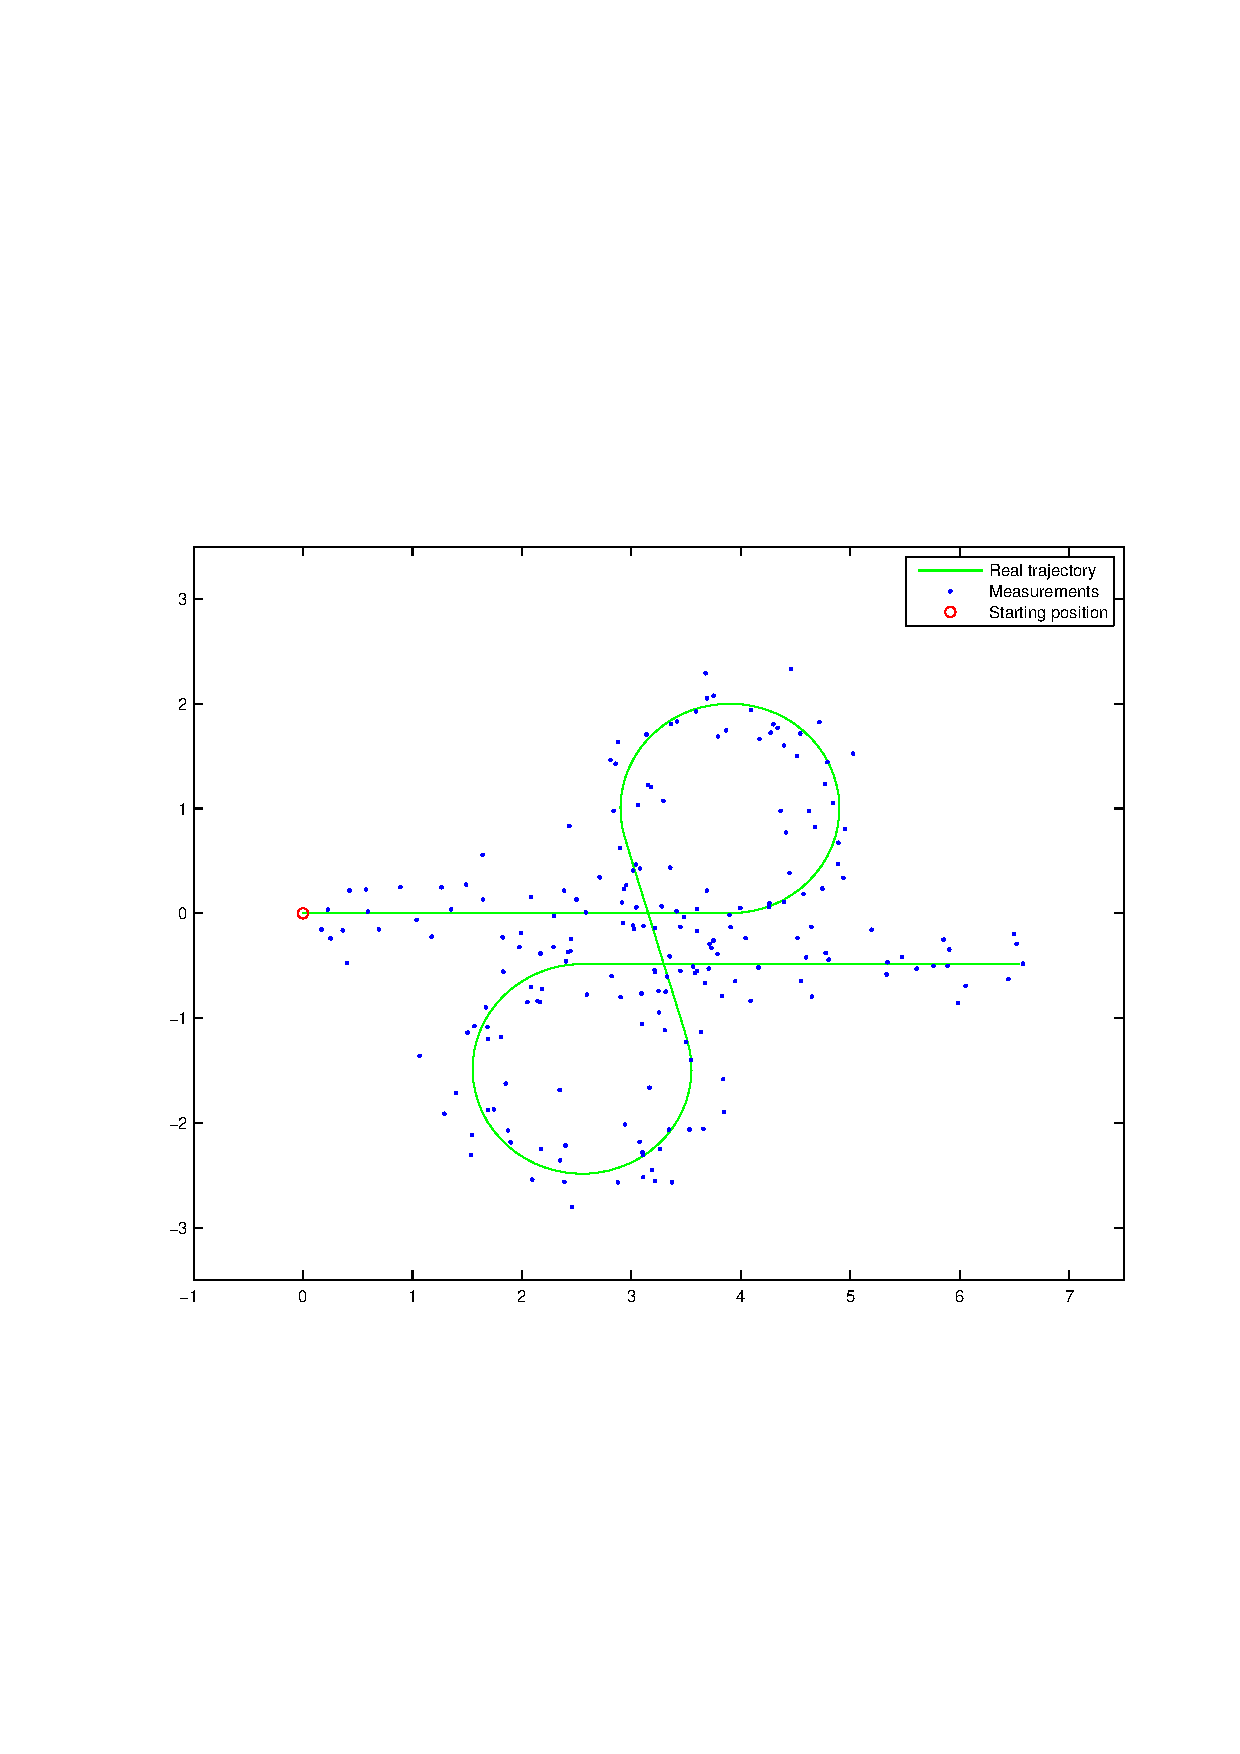
\includegraphics[width=11cm]{pics/eimm1_trajectory}
\caption{ Object's trajectory and a sample of measurements in the
Coordinated turn model demonstration.  }
\label{fig:eimm1_trajectory}
\end{center}
\end{figure}

\begin{figure}
\begin{center}
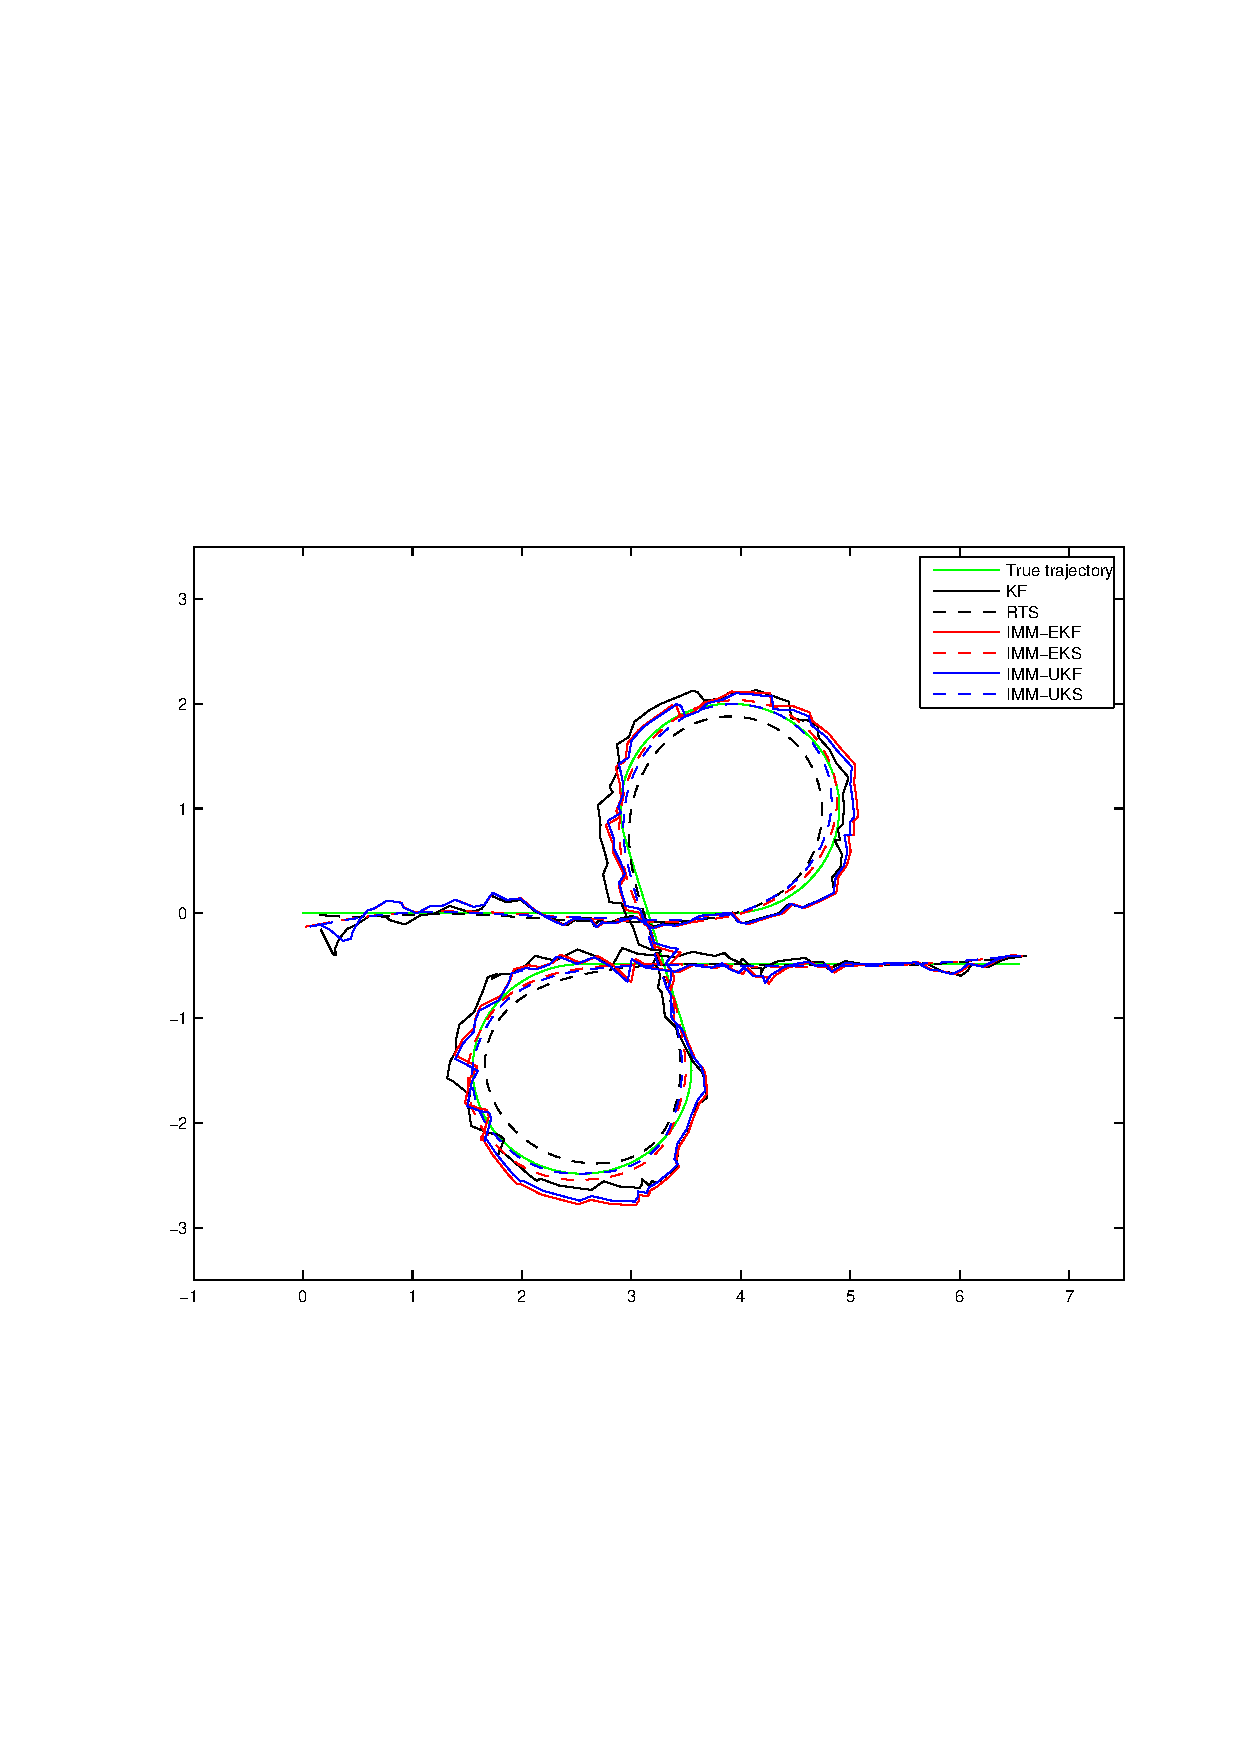
\includegraphics[width=11cm]{pics/eimm1_1}
\caption{ Position estimates in the Coordinated turn model
demonstration.  }
\label{fig:eimm1_1}
\end{center}
\end{figure}

\begin{figure}
\begin{center}
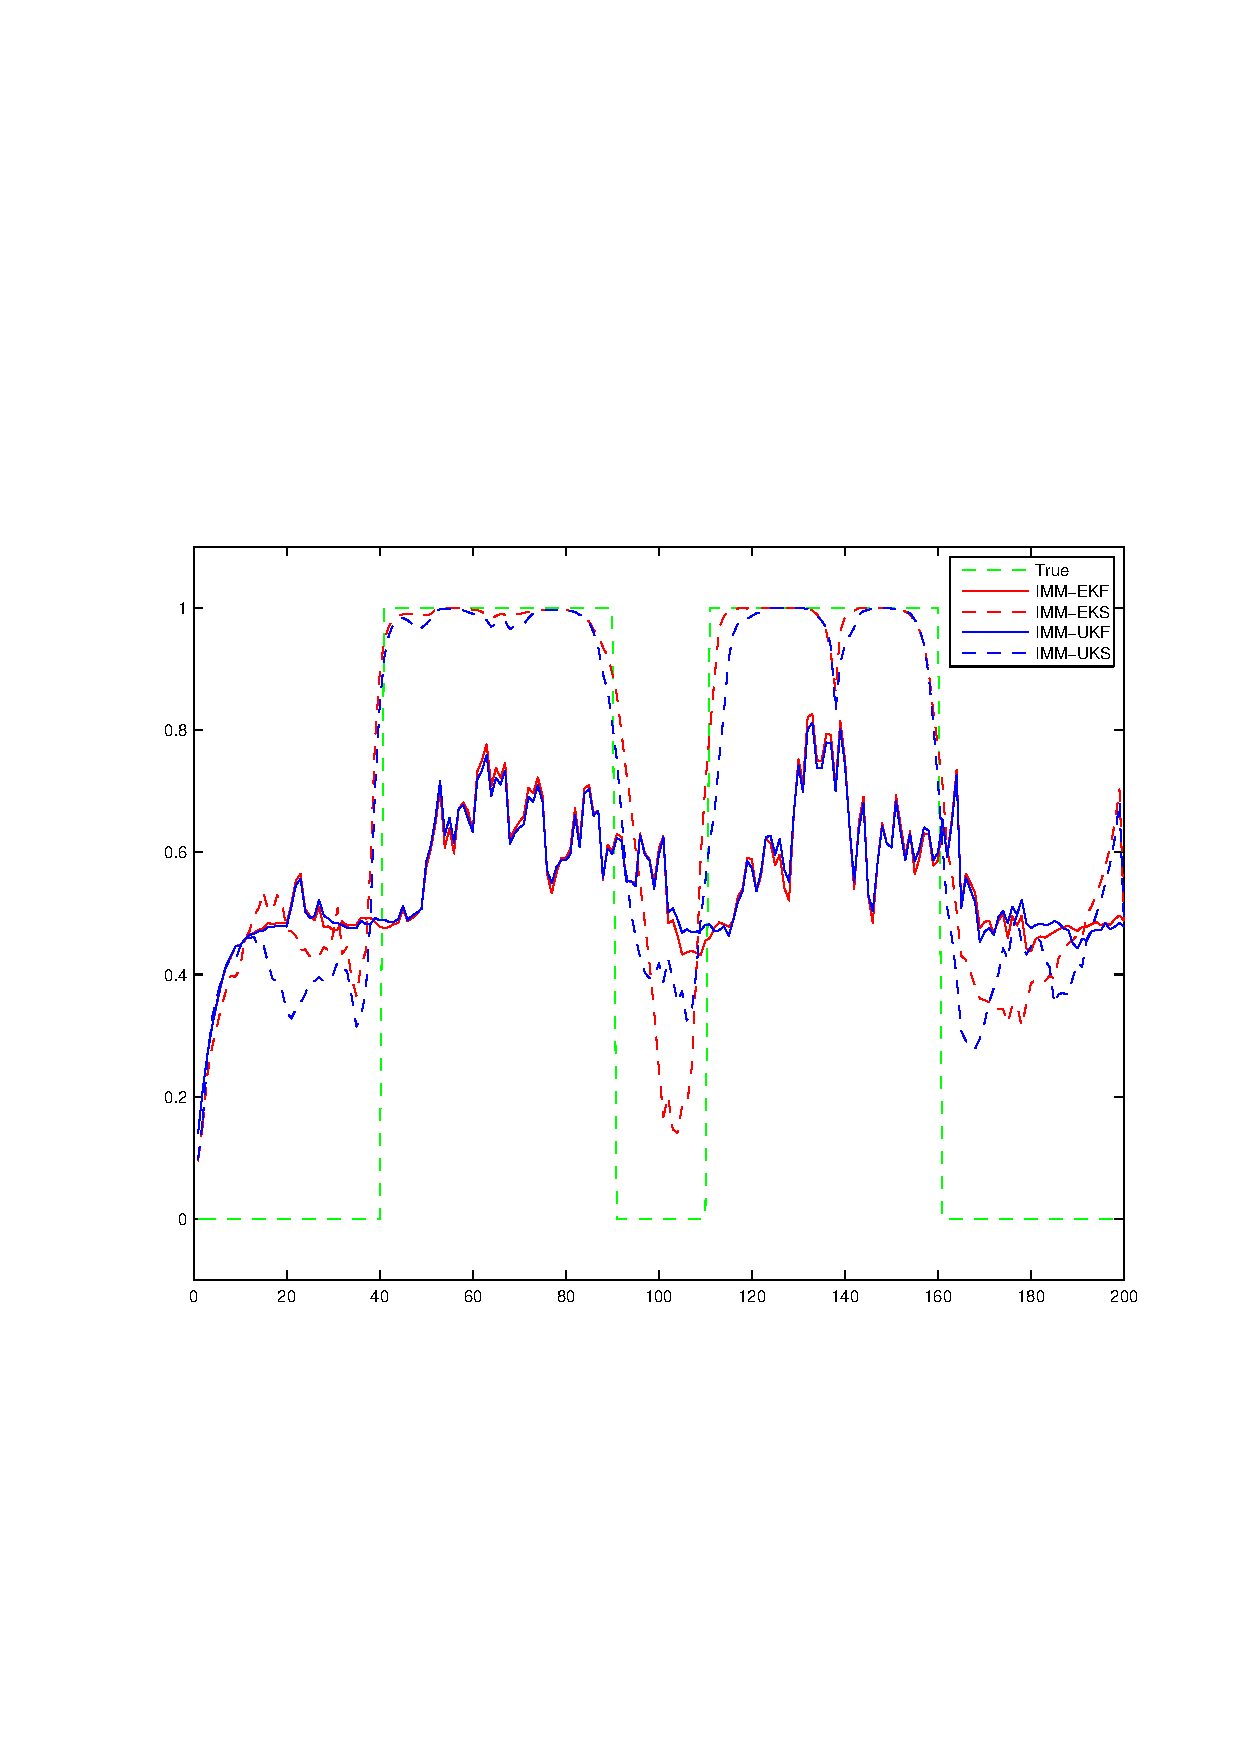
\includegraphics[width=11cm]{pics/eimm1_2}
\caption{ Estimates for model 2's probability in Coordinated turn
model demonstration.  }
\label{fig:eimm1_2}
\end{center}
\end{figure}

\begin{figure}
\begin{center}
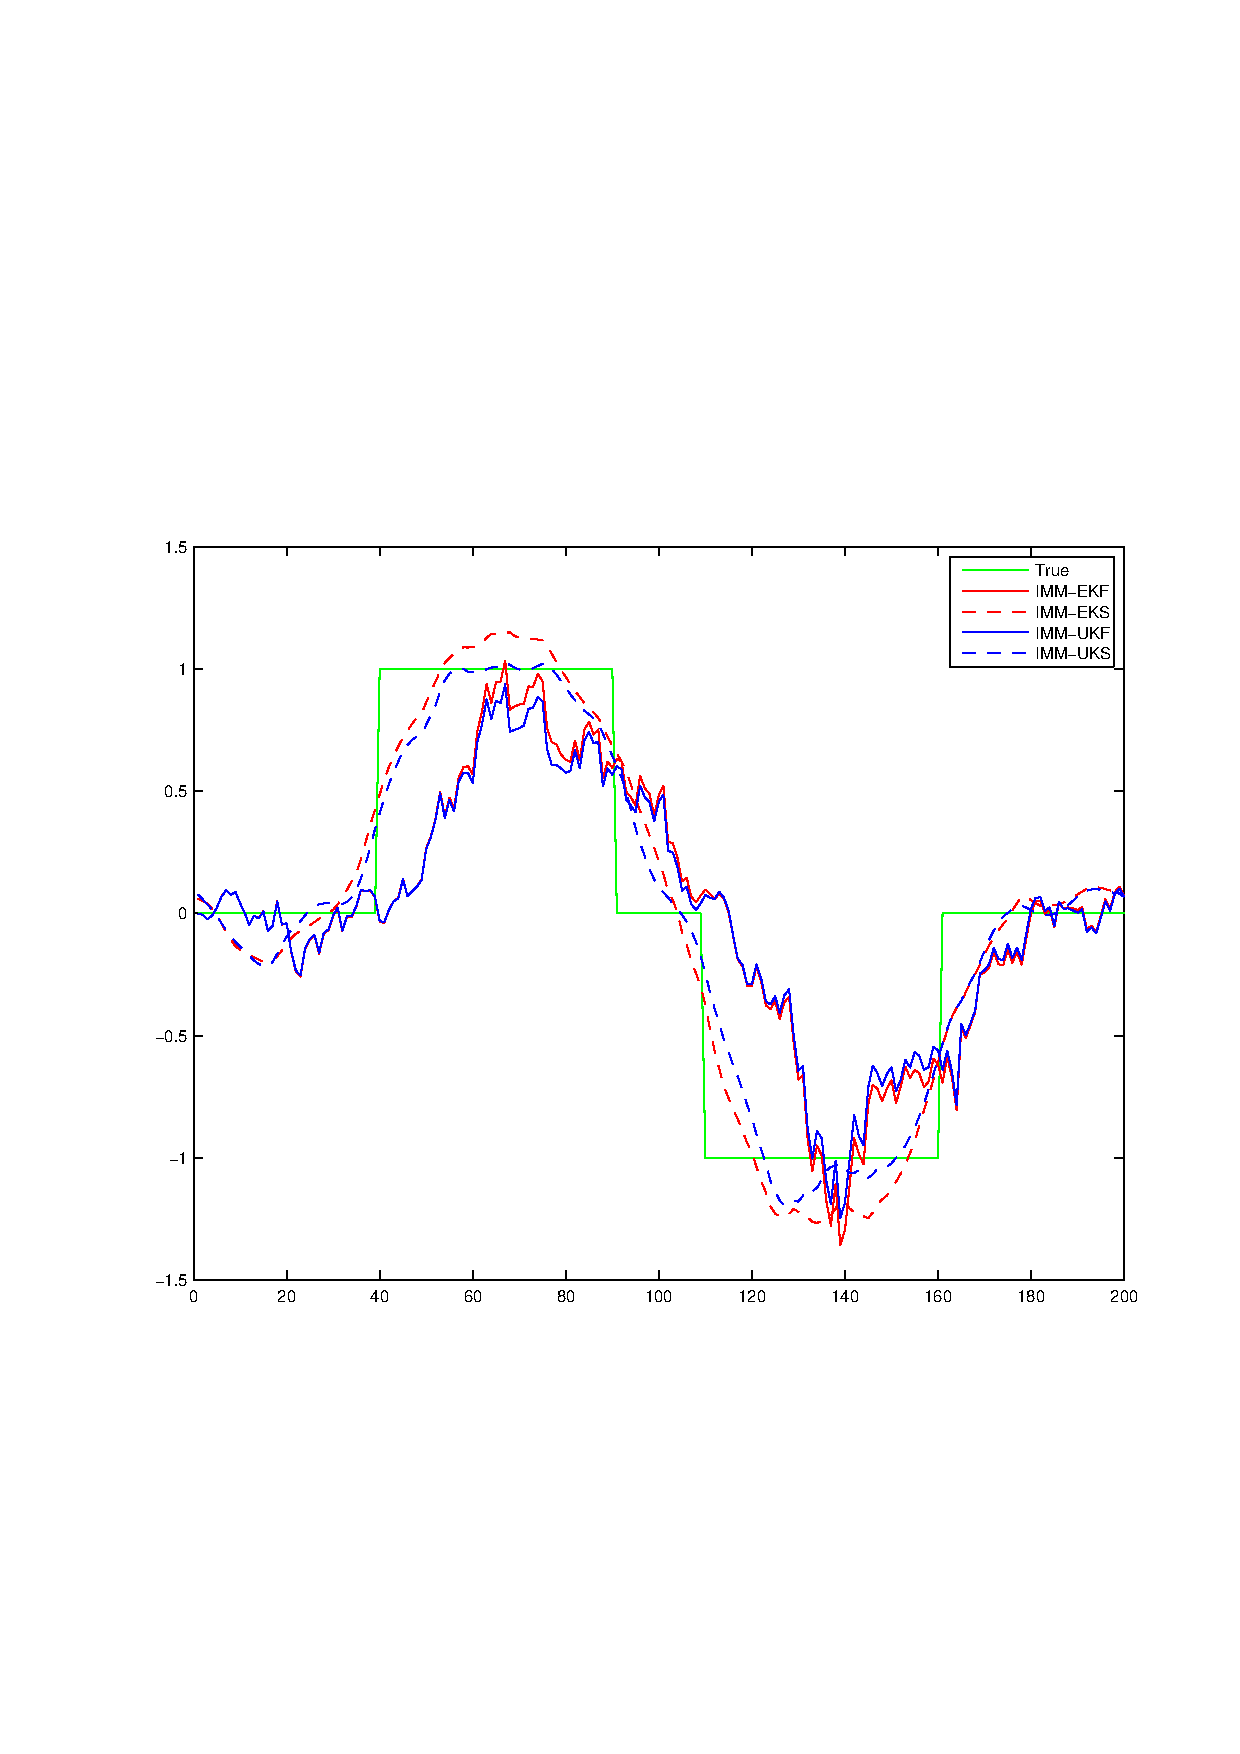
\includegraphics[width=11cm]{pics/eimm1_3}
\caption{ Estimates of the turn rate parameter $\omega_k$ in the
Coordinated turn model demonstration.  }
\label{fig:eimm1_3}
\end{center}
\end{figure}

%  
\begin{table}
\begin{center}
\begin{tabular}{|l|l|} \hline {\it Method}&{\it MSE } \\ \hline KF &
0.0253 \\ KS & 0.0052 \\ EIMM1 & 0.0179 \\ EIMMS1 & 0.0039 \\ UIMM1 &
0.0155 \\ UIMMS1 & 0.0036 \\ \hline
\end{tabular}
\caption{Average MSEs of estimating the position in Tracking Object
with Simple Manouvers example over 100 Monte Carlo runs.}
\label{table:eimm1_mse}
\end{center}
\end{table}
%

\subsection{Demonstration: Bearings Only Tracking of a Manouvering
Target}

We now extend the previous demonstration by replacing the linear
measurement model with a non-linear bearings only measurement model,
which were reviewed in section 2.2.9. The estimation problem is now
harder as we must use a non-linear version of IMM filter update step
in addition to the prediction step, which was used in the previous
demonstration.

The trajectory of the object is exactly the same as in the previous
example. The sensors producing the angle measurements are located in
$(s_x^1,s_y^1) = (-0.5,3.5)$, $(s_x^2,s_y^2) = (-0.5,3.5)$,
$(s_x^3,s_y^3) = (7,-3.5)$ and $(s_x^4,s_y^4) = (7,3.5)$. The
trajectory and the sensor positions are shown in figure
\ref{fig:eimm2_trajectory}.  The standard deviation of the
measurements is set to $\sigma = 0.1$ radians, which is relatively
high.

\begin{figure}
\begin{center}
\includegraphics[width=11cm]{pics/eimm2_trajectory}
\caption{ Object's trajectory and positions of the sensors in Bearings
Only Tracking of a Manouvering Target demonstration.  }
\label{fig:eimm2_trajectory}
\end{center}
\end{figure}

The function call of IMM-EKF update step is of form
%
\begin{lstlisting} 
[x_ip,P_ip,mu_ip,m,P] = eimm_update(x_p,P_p,c_j,ind,dims, ...
  Y(:,i),H,h_func,R,h_param);
\end{lstlisting}
%
which differs from the standard IMM filter update with the additional
parameters \texttt{h} and \texttt{h\_param}, which contain the handles
to measurement model functions and their parameters,
respectively. Also, the parameter \texttt{H} now contains the handles
to functions calculating the Jacobian's of the measurement
functions. In IMM-UKF the update function is specified similarly.

The position of the object is estimated with the following methods:
\begin{itemize}
\item EKF and EKS: Extended Kalman filter and (RTS) smoother using the
same Wiener process velocity model as in the previous demonstration in
the case standard Kalman filter.
\item UKF and UKS: Unscented Kalman filter and (RTS) smoother using
the same model as the EKF.
\item IMM-EKF and IMM-EKS: EKF based IMM filter and smoother using the
same combination of Wiener process velocity model and a coordinated
turn model as was used in the previous demonstration in the case of
IMM-EKF and IMM-UKF.
\item IMM-UKF and IMM-UKS: UKF based IMM filter and smoother using the
same models as IMM-EKF.
\end{itemize}
%
A sample of trajectory estimates are plotted in figure
\ref{fig:eimm2_1}. The estimates are clearly more inaccurate than the
ones in the previous section. In figure \ref{fig:eimm2_2} we have
plotted the estimates of model 2's probability for IMM-EKF and
IMM-UKF. The figure look very similar to the one in the previous
demonstration, despite the non-linear and more noisy
measurements. Also the turn rate estimates, which are plotted in
figure \ref{fig:eimm2_3}, are very similar to the ones in the previous
section with exception that now the difference between the smoothed
estimates of IMM-EKF and IMM-UKF is bigger.

\begin{figure}
\begin{center}
\includegraphics[width=11cm]{pics/eimm2_1}
\caption{ Filtered and smoothed estimates of object's position using
all the tested methods in Bearings Only Tracking of a Manouvering
Target demonstration.  }
\label{fig:eimm2_1}
\end{center}
\end{figure}

\begin{figure}
\begin{center}
\includegraphics[width=11cm]{pics/eimm2_2}
\caption{ Estimates for model 2's probability in Bearings Only
Tracking of a Manouvering Target demonstration.  }
\label{fig:eimm2_2}
\end{center}
\end{figure}

\begin{figure}
\begin{center}
\includegraphics[width=11cm]{pics/eimm2_3}
\caption{ Estimates for the turn rate parameter $\omega_k$ in Bearings
Only Tracking of a Manouvering Target demonstration }
\label{fig:eimm2_3}
\end{center}
\end{figure}

In table \ref{table:eimm_rmse2} we have listed the average mean square
errors of position estimates over 100 Monte Carlo runs.  It can be
observed that the estimates of EKF and UKF are identical in practice,
which is to be expected from Bearings Only Tracking demonstration. The
difference between IMM-UKF and IMM-EKF has grown in the favor of
IMM-UKF, whereas the accuracy of IMM-EKF is now more close to the ones
of EKF and UKF. On the other hand the smoothed estimates of IMM-UKF
and IMM-EKF are still very close to one another, and are considerably
better than the smoothed estimates of EKF and UKF.

%  
\begin{table}
\begin{center}
\begin{tabular}{|l|l|} \hline {\it Method}&{\it MSE } \\ \hline EKF &
0.0606 \\ ERTS & 0.0145 \\ UKF & 0.0609 \\ URTS & 0.0144 \\ IMM-EKF &
0.0544 \\ IMM-EKS & 0.0094 \\ IMM-UKF & 0.0441 \\ IMM-UKS & 0.0089 \\
\hline
\end{tabular}
\caption{Average MSEs of estimating the position in Bearings Only
Tracking of a Manouvering Target example over 100 Monte Carlo runs.}
\label{table:eimm_rmse2}
\end{center}
\end{table}
%

It should be noted that the performance of each tested method could be
tuned by optimizing their parameters (e.g. variance of process noise
of dynamic models, values of model transition matrix in IMM etc.)
more carefully, so the performance differences could change
radically. Still, it is clear that IMM filter does actually work also
with (atleast some) non-linear dynamic and measurement models, and
should be considered as a standard estimation method for multiple
model systems. Also, one should prefer IMM-UKF over IMM-EKF as the
performance is clearly (atleast in these cases) better, and the
implementation is easier, as we have seen in the previous examples.

